\documentclass{exam}

\usepackage{units} 
\usepackage[fleqn]{amsmath}
\usepackage{float}
\usepackage{mdwlist}
\usepackage{booktabs}
\usepackage{caption}
\usepackage{fullpage}
\usepackage{enumerate}
\usepackage{graphicx}

\usepackage{2in1, lscape} 

\everymath{\displaystyle}

\author{}
\date{January 22, 2014}
\title{Statistics \\ Week One}

\begin{document}

\maketitle
\tableofcontents

  \section{NFL}

  \subsection{Passing Attempts vs. Yards}

  \begin{table}[ht]
    \centering
    \begin{tabular}{lrrrrrrrrrr}
      \toprule
      PA & 22  & 56  & 31  & 37  & 27  & 38  & 40  & 22  & 27  & 26 \\
      PY & 100 & 428 & 206 & 169 & 206 & 207 & 284 & 208 & 261 & 220 \\
      \midrule
      PA & 20  & 50  & 27  & 53  & 28  & 34  & 39  & 57  & 35  & 46 \\
      PY & 120 & 388 & 421 & 399 & 269 & 295 & 201 & 419 & 234 & 300 \\
       \bottomrule
    \end{tabular}
    \caption{Passing attempts vs. yards}
  \end{table}

  \begin{figure}[H]
    \centering
    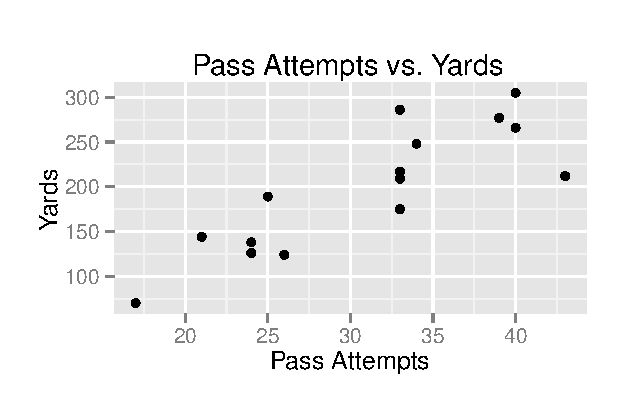
\includegraphics{figures/nfl/passing_attempts_vs_yds.eps}
    \caption{Passing attempts vs. yards}
  \end{figure}

  \[
    c = 0.7225
  \]

\end{document}

